\documentclass[a4paper,11pt]{article}
\usepackage[utf8]{inputenc}
\usepackage[T1]{fontenc}
\usepackage[french]{babel}
\usepackage[right=2.5cm, left=2.5cm, bottom=4cm, top=3cm]{geometry}
\usepackage[ddmmyyyy]{datetime}
\usepackage[table]{xcolor}
\usepackage{lmodern,mathptmx,changepage,titlesec,hyperref,listings,lstautogobble,graphicx,array,longtable,multirow,lipsum,tikz,shorttoc,enumitem,float}
\usetikzlibrary{arrows,automata}
\usetikzlibrary{positioning}

\renewcommand{\rmdefault}{\sfdefault} %Utilisation de la police sans-serif ("Computer Modern Sans") pour la police roman
\renewcommand{\ttdefault}{pcr} 	%Utilisation d'une police "CourrierNew" pour la police monospaced (pour faire un listing manuel)
\linespread{1.15}				%Interligne

%Utilisation de liens colorés en bleu et soulignés
\hypersetup{colorlinks=true, urlcolor=blue, urlbordercolor=blue, linkcolor=black, linkbordercolor=white}
\makeatletter \Hy@AtBeginDocument{\def\@pdfborder{0 0 1} \def\@pdfborderstyle{/S/U/W 1}}\makeatother

\titlespacing*{\section} {0cm}{7ex plus 1ex minus .2ex}{1.5ex plus .2ex}
\titlespacing*{\subsection} {0cm}{4.5ex plus 1ex minus .2ex}{1.5ex plus .2ex}
\titleformat*{\section}{\LARGE\bfseries}
\titleformat*{\subsection}{\large\bfseries}
\titleformat*{\subsubsection}{\normalsize\bfseries}

\definecolor{darkgreen}{rgb}{0,0.8,0}
\definecolor{mygray}{rgb}{0.93,0.93,0.93}
\definecolor{mymauve}{rgb}{0.58,0,0.82}
\lstset{	
	language=Python,
	basicstyle=\small\ttfamily,
	backgroundcolor=\color{mygray},
	breaklines=true,
	breakatwhitespace=true,
	tabsize=3,
	frame=none,
	rulecolor=\color{black},
	keywordstyle=\color{blue}\bfseries,
	stringstyle=\color{orange},
	showstringspaces=false,
	commentstyle=\footnotesize\color{darkgreen},
	keepspaces=true,
	extendedchars=true,
	numbers=left,
	numberstyle=\tiny\color{lightgray},
	stepnumber=1,
	escapeinside={(@}{@)},
	autogobble=true,
	literate=
		{á}{{\'a}}1 {é}{{\'e}}1 {í}{{}}1 {ó}{{\'o}}1 {ú}{{\'u}}1
		{Á}{{\'A}}1 {É}{{\'E}}1 {Í}{{\'I}}1 {Ó}{{\'O}}1 {Ú}{{\'U}}1
		{à}{{\`a}}1 {è}{{\`e}}1 {ì}{{\`i}}1 {ò}{{\`o}}1 {ù}{{\`u}}1
		{À}{{\`A}}1 {È}{{\'E}}1 {Ì}{{\`I}}1 {Ò}{{\`O}}1 {Ù}{{\`U}}1
		{ä}{{\"a}}1 {ë}{{\"e}}1 {ï}{{\"i}}1 {ö}{{\"o}}1 {ü}{{\"u}}1
		{Ä}{{\"A}}1 {Ë}{{\"E}}1 {Ï}{{\"I}}1 {Ö}{{\"O}}1 {Ü}{{\"U}}1
		{â}{{\^a}}1 {ê}{{\^e}}1 {î}{{\^i}}1 {ô}{{\^o}}1 {û}{{\^u}}1
		{Â}{{\^A}}1 {Ê}{{\^E}}1 {Î}{{\^I}}1 {Ô}{{\^O}}1 {Û}{{\^U}}1
		{œ}{{\oe}}1 {Œ}{{\OE}}1 {æ}{{\ae}}1 {Æ}{{\AE}}1 {ß}{{\ss}}1
		{ç}{{\c c}}1 {Ç}{{\c C}}1 {ø}{{\o}}1 {å}{{\r a}}1 {Å}{{\r A}}1
		{€}{{e}}1 {£}{{\pounds}}1 {«}{{\guillemotleft}}1
		{»}{{\guillemotright}}1 {ñ}{{\~n}}1 {Ñ}{{\~N}}1 {¿}{{?`}}1
}

%Redéfinition de la taille de \Huge pour le titre du document
\makeatletter\renewcommand\Huge{\@setfontsize\Huge{37pt}{40}}\makeatother
\date{\today}


\title{\vspace{\fill}\textbf{\Huge Rapport}}
\author{Jean-Didier Pailleux - Maxence Joulin - Damien Thenot - Romain Robert - Robin Feron 
	\vspace{2em}\\
	\textit{Test de primalité}\\
	\textcolor{red}{https://github.com/CHPS-M1-PRIME-NUMBERS/Prime\_numbers}
	\vspace{2em}
}

\begin{document}
\pagenumbering{gobble}\clearpage
\maketitle\vspace{13em}
\begin{center}
\includegraphics[scale=0.7]{logo.png}\end{center}
\begin{flushright}\textit{Projet de Programmation numérique}\end{flushright}
\newpage
\tableofcontents
\newpage\clearpage\pagenumbering{arabic}

	\section{Introduction}
% pour l'intro si tu modifies des trucs, garde la meme mise en page malek.
	\paragraph{}Ce document est le compte-rendu de notre travail qui s'inscrit dans le cadre du module \textit{Projet de Programmation numérique} du master \textit{Calcul Haute Performance Simulation} de l'\textit{\textbf{UVSQ}}. Le sujet de ce projet a été proposé par l'encadrant Sébastien Gougeau.
	
	\paragraph{}Ce projet découle d'un thème qui est le test de primalité, et consiste à tester si un nombre est bien premier ou non. Un nombre premier est un entier qui admet uniquement deux diviseurs distincts et positifs (1 et lui même). 
	Les nombres premiers prennent une place importante dans le domaine des mathématiques et ont des propriétés très utiles particulièrement dans le domaine de la cryptographie. La recherche de très grands nombres premiers est devenu de plus en plus captivé par beaucoup, de nombreux tests de primalité ont pu émerger, voir évoluer, devenir plus performants, et de plus en plus rapides.
	
	\paragraph{}Il existe actuellement deux types de tests de primalités, les déterministes qui permettent d'établir avec certitude le résultat et les tests probabilistes qui émettent un résultat n'ont fiable avec une certaine probabilité d'erreur mais sont plus rapide que les tests déterministes.
	
	\paragraph{}L'objectif de ce projet consiste à implémenter plusieurs de ces tests (déterministes) et ainsi comparer leur vitesse  d'exécution. Ceci et pour une exécution sur le test de primalité pour un nombre premier, et pour une exécution sur le test de n nombres premiers. De plus un test probabiliste sera programmer pour ainsi comparer la fiabilité du résultat et le temps que nécessite de faire cet algorithme.\\ 
	Une partie bonus nous a été proposé lors de notre entretient avec Monsieur Gougeau qui consiste à implémenter une fonctionnalité pour déterminer si un nombre est hautement composé (c'est à dire que le nombre de ses diviseurs est supérieur strictement à tout les nombres inférieur lui). 
	
	\paragraph{}Dans la première partie de ce document, on présentera l'architecture de notre projet (la décomposition), illustrée par un organigramme qui a été préalablement établi.\\
	Après cela, on mentionnera les différents outils et langages utilisé au cours de la phase l'implémentation.\\
	Puis dans une autre partie l'analyse des résultats établis lors des tests du projet accompagné d'un comparatif de la performance des tests.\\
	Finalement, dans les deux dernières parties, on établira un bilan quant à l'organisation interne au sein du groupe et un bilan technique du projet qui mettra en avant les limites de chaque test de primalité.
	
		
	\section{Architecture du projet}
		\subsection{Organigramme}
		L'organigramme suivant fait part de la décomposition que va adopter le projet. Le projet se décompose en trois catégories de tests pour les nombres hautement composé, les tests de primalité déterministe et les tests de primalité probabiliste. \\ 
		\begin{center}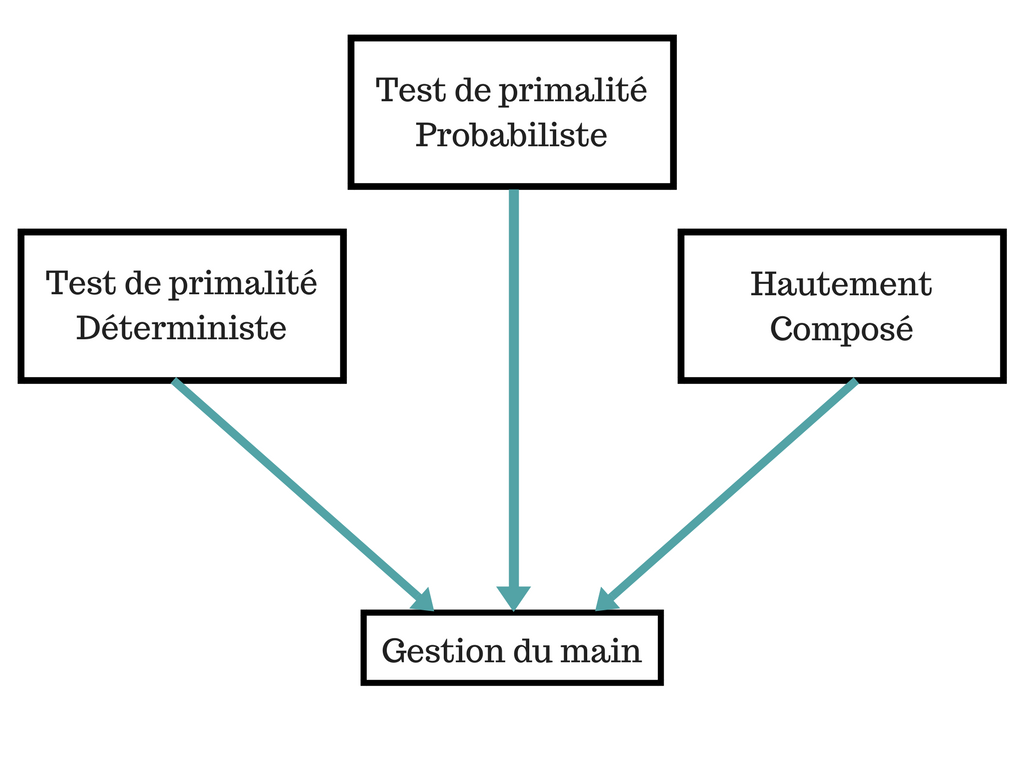
\includegraphics[scale=0.5]{organigramme.png}\end{center}
		
		\subsection{Tests de primalité}
		Au cours de ce projet il nous a été demandé d'implémenter plusieurs algorithme pour déterminer si un nombre est premier ou non. Voici les différents tests utilisés pour ce travail:
		\begin{itemize}
			\item Méthode naïve le \textbf{crible d’Ératosthène}\footnote{zanotti.univ-tln.fr/ALGO/I51/Crible.html} utilisé pour le memory bound. Cet l'algorithme va procéder à une élimination dans une table d'entiers de 2 à N de tous les multiples de chaque entier présent dans ce tableau. En supprimant tous les multiples à la fin seuls les entiers qui ne sont multiples d'aucun autre resteront, et par conséquent ces nombres seront donc premiers. Le memory bound va donc être une liste des entiers restant à la fin de l'application du crible.\\
			
			\item Méthode naïve \textbf{l'algorithme d'Euclide} (Déterministe).\\
			
			\item \textbf{Pocklington} (Déterministe): Le test de primalité de Pocklington-Lehmer utilise le théorème de Pocklington pour vérifier la primalité d’un nombre.
L’algorithme consiste à utiliser une factorisation partielle du nombre N-1, où N est le nombre dont on souhaite tester la primalité. Cette factorisation partielle nous permet d’obtenir un nombre que l’on nommera A et qui doit remplir certaines conditions pour qu’on puisse appliquer le théorème.
Nous avons déjà la factorisation de A qui nous servira pour la suite de l'exécution de l’algorithme. 
La suite consiste à tester les conditions requises sur tous les facteurs premiers de A, ces conditions sont de trouver un nombre "$a$" qui mis à la puissance N-1 modulo N donne 1 et que le plus grand diviseur commun entre {\Large$\frac{a^{(N-1)}}{p}$} et N soit égal à 1, avec p le facteur premier de A tester en ce moment. Si on a trouvé un "$a$" remplissant les conditions pour chaque “p” alors on peut dire que le nombre N est premier.\\

			\item \textbf{AKS}\footnote{https://en.wikipedia.org/wiki/AKS\_primality\_test} 2002 (Déterministe)\\
			
			\item \textbf{Miller-Rabin} (Probabiliste): Miller-Rabin, basé sur le petit théorème de Fermat \\ $a^p-1 \equiv 1 \pmod p$, consiste à tirer parti d'une équation ou d'un système d'équations qui sont vraies pour des valeurs premières, et à regarder si elles sont toujours vraies ou non pour un nombre dont nous voulons tester la primalité. La fonction Miller-Rabin prend en paramètre un entier n dont on souhaite vérifier la primalité et un entier k qui représente le nombre d’itération du test de Miller-Rabin plus k est élevé est plus l’analyse est précise (moins de chance d’erreurs).\\
		\end{itemize}
		
		\subsection{Nombres Hautement composés}
		Deux fonctions ont été implémenté pour les nombres hautement composés. La première fonction : 				\begin{lstlisting}
			bool highly_composite_naive(unsigned int number)
		\end{lstlisting}
		C'est une méthode naïve qui consiste à calculer le nombre de diviseur d'un nombre n et de comparer ce nombre avec le nombre de diviseurs pour tout entier k compris entre $1$ et $n-1$.
		\paragraph{}La seconde fonction est :
		\begin{lstlisting}
			bool highly_composite_def(unsigned int number)
		\end{lstlisting}
		Elle utilise la propriété sur la forme qu'un nombre hautement composé doit avoir. Un nombre hautement composé possèdent des facteurs premiers les plus petits possible. Si l'on doit prendre en considération que la décomposition d'un entier $n > 1$ en produit de facteurs premiers comme suit  $n = p_1^{c_1} * p_2^{c_2} * ... * p_k^{c_k}$ où $p_1 = 2 < p_2 = 3 < … < p_k$ sont les $k$ plus petits nombres premiers, avec $c_k$ le dernier exposant non nul.
		\paragraph{}En conséquence, pour que n soit hautement composé, il faut que $c_1 \ge c_2 \ge ... \ge c_k$. En cas de non respect de cette règle si nous échangeons deux exposants on diminue le nombre n tout en conservant exactement le même nombre de diviseurs. Un exemple pour illustrer : 18 = $2^1 * 3^2$ peut être remplacé par $12 = 2^2 * 3^1$, ces deux nombres ont tout les deux 6 diviseurs). De plus il a été montré que le dernier exposant $c_k = 1$, sauf dans deux cas particuliers $n = 4$ et $n = 36$.

	\section{Outils et langages de programmation}
		\subsection{Langages de programmation}
		Lors de la réalisation du projet, des contraintes nous ont été imposées par notre encadrant. Tout d'abord, le langage de programmation utilisé est le langage C++. Langage adapté pour la programmation procédurale et pour la programmation orientée objet. De plus, il dispose de nombreuses bibliothèques permettant de manipuler des grands entiers supérieur à $2^{64}$, de chronométrer l'exécution d'une portion du programme, et autre.\\
		Le deuxième langage est le Shell. Celui-ci faisant partie du système d'exploitation UNIX, va nous permettre d'établir un script \textit{test.sh} avec l’enchaînement de plusieurs lignes de commandes pour l'exécution de tests.
		
		\subsection{Outils}
		Pour ainsi produire le projet certains outils ont été utilisé pour obtenir le résultat présenté. En premier lieu nous avons utilisé la bibliothèque \textit{GMP}.  Cette dernière est une bibliothèque qui va permettre de générer de très grands nombre car les types de base proposé par le C++ nous limite à l'utilisation de nombre de 64 bits maximum.
		\paragraph{}Ensuite le second outils utilisé est la bibliothèque \textit{NTL}, propose certaines fonctionnalité pour le calcul du PolyModulo\footnote{https://en.wikipedia.org/wiki/AKS\_primality\_test} qui nous est indispensable pour l'implémentation du test de primalité AKS. N'ayant aucune connaissance nécessaire dans le domaine mathématique sur le polymodulo, l'utilisation de cette bibliothèque nous permet d'obtenir des fonctions pour ces calculs et de façon optimisée.  
		\paragraph{}Nous avons également utilisé un service d’hébergement de gestion de développement utilisant le système de gestion de version \textit{Git} qui est \textbf{GitHub}. Ceci nous a permis de travailler en groupe sur un dépôt de façon très facile tout en étant indépendant lorsque chacun devait travailler de son côté sur une fonctionnalité sans pour autant perturber le travail du reste du groupe. GitHub nous permet également de stocker les différentes versions de notre travail.   
		\paragraph{}Enfin le dernier outilsutilisé est \textit{Cmake}\footnote{https://cmake.org/}. CMake est une famille d'outils multi-plateformes et open source permettant de construire, tester et emballer des logiciels. Nous l'utilisons pour la compilation du projet, la liaison avec plusieurs bibliothèques utilisées et pour la génération d'un makefile. 
			
	\section{Analyse des résultats}
	Dans cette partie nous allons donc analyser les résultats obtenus lors des tests et les comparer entres elles. En premier lieu nous avons tester chaque test de primalité sur un nombre N premier très grand, les faires tourner sur un nombre d'itération $iter$ pour obtenir une moyenne sur du temps d'exécution pour chaque algorithme. \\
	
		\textbf{METTRE LE PLOT - LE N du test - iter du test - COMMENTAIRE DES RESULTATS}\\ 
	
	\section{Bilan Technique du Projet}	
		Après l'analyse des résultats nous pouvons constater que les différents tests appliqués possèdent chacun des limites.	
		Tout d'abord, la principale limite du crible d'Eratosthène concerne la taille de son tableau. En effet, pour un nombre N très très grand, le crible va créer un tableau de booléen de taille N+1, ce qui va prendre énormément de place en mémoire. Puis pour la création de la liste contenant les nombres premiers de 2 jusqu'à N, la fonctionnalité de memory\_bound va devoir parcourir toute les cases du tableau du crible pour remplir sa liste, ce qui engendre une complexité de N pour cette opération de remplissage.\\
		
		Ensuite, pour le test de Pocklington la limite principale est le besoin de factoriser le voisin d’en dessous du nombre dont on cherche à valider la primalité, c’est-à-dire N-1 si N est le nombre dont on met la primalité en question. La factorisation des grands nombres est une lourde tâche de calcul de difficulté exponentielle, ainsi même les programmes les plus efficaces demandent énormément de temps, des années voir plus, pour factoriser certaines nombres très grands.
En réalité, nous avons la possibilité de factoriser N-1 qu’en partie, il suffit de factoriser N-1 jusqu’à trouver un A créer à partir des facteurs premiers de N-1 qui respecte les conditions nécessaires pour appliquer le théorème.\\

					
	\section{Organisation interne du groupe}
	Pour débuter la programmation de ce projet, il nous fallait en premier lieu établir la répartition du travail de groupe pour que le projet puisse avancer de façon efficace et de manière rapide. Le tableau ci-dessus va ainsi indiquer pour chaque membre du groupe la ou les fonctionnalités pour laquelle il a pu contribuer à l'élaboration: \\
	
	\begin{center}\vspace{-1em}\footnotesize\begin{longtable}{|>{\centering}m{4cm}|>{\centering}m{2cm}|>{\centering}m{2cm}|>{\centering}m{2cm}|>{\centering}m{2cm}|>{\centering\arraybackslash}m{2cm}|}			
		\hline \multicolumn{1}{|c|}{\textbf{Tâches}} & \multicolumn{1}{c|}{\textbf{Jean-Didier}} & \multicolumn{1}{ c|}{\textbf{Maxence}} & \multicolumn{1}{ c|}{\textbf{Romain}} & \multicolumn{1}{ c|}{\textbf{Robin}} & \multicolumn{1}{c|}{\textbf{Damien}}\\
		\hline 	Eratosthène/Memory Bound & x & ~ & ~ & ~ & ~ \\
		\hline 	Euclide/Computation Bound & ~ & x & ~ & ~ & ~ \\
		\hline 	AKS & ~ & ~ & x & ~ & ~ \\
		\hline 	Pocklington & ~ & ~ & ~ & ~ & x \\
		\hline 	Miller-Rabin & ~ & ~ & ~ & x & ~ \\
		\hline 	Highly Composite & x & ~ & ~ & ~ & ~ \\
		\hline 	Cmake  & x & x & ~ & ~ & ~ \\
		\hline  Script & x & ~ & ~ & ~ & ~ \\
		\hline
	\end{longtable}\vspace{-2.2em}\end{center}	

	\section{Conclusion}

\end{document}